\subsection{Description de l'espace de clef}
\par Pour mieux comprendre la structure de donnée dans cassandra
cette partie propose un petit point sur ce qu'est un espace de clef,
une brève définition et une comparaison avec d'autre systemes connus.
On propose également de décrire la commande de création proposé dans le TP: \newline

\begin{tt}
\begin{alltt}
cqlsh> CREATE KEYSPACE TP WITH REPLICATION = \{
\indent		'class' : 'SimpleStrategy',
\indent		'replication\_factor' : '1'
\};
\end{alltt}
\end{tt}

\textcolor{ForestGreen}{\textbf{Definition}}(Keyspace): Il s'aggit de la plus grande structure de données de cassandra. Elle est comparable aux bases (ou schéma)
dans les systemes classiques ou dans les systèmes document (mongodb, couchdb). Elle contient des familles de colonnes,  qui elles, représentent
la séparation entre les tables (mysql) ou les collections (mongodb). Chaque ligne insérée présente des informations pour certaines colonnes
d'un famille de colonnes.

\begin{block}{Propriétées}
\begin{itemize}
\item \textbf{Replication factor}: définit le nombre de noeud possédant un copie de la donnée. 
\item \textbf{Replica placement strategy}: il s'agit du mode de répartition des réplicats. Il en 
existe trois. simple strategy,  old network topology strategy, network topology strategy
\item \textbf{Column families}: Liste des familles des colonnes associées. Dans notre cas sur le keyspace
TP il y a user, follows et message.
\end{itemize}
\end{block}

\par La commande de création du Keyspace TP signifie donc: créer l'espace de clefs TP dont les lignes ne sont présentes que sur un noeud.
Si il doit y avoir de la réplication le \textit{partitioner} rédistrubura automatiquement sur le noeud suivant.\newline La commande DESCRIBE nous permet d'avoir la liste de keyspaces.\newline
\begin{tt} 
\indent cqlsh> DESCRIBE KEYSPACES; \newline 
\indent system\_traces  OpsCenter  system  \textcolor{red}{tp}\end{tt}\newline \newline
On peut ensuite accéder aux familles de colonnes sur un espace de clefs particulier.\newline
\begin{tt}
\indent cqlsh> use TP; \newline 
\indent cqlsh:tp> DESCRIBE TABLES;\newline 
\indent follows  message  user\end{tt}\newline \newline
On peut ensuite retrouver les colonnes d'une famille en particulier. \newline
\begin{tt}
\indent cqlsh:tp> DESCRIBE TABLE user; \newline 
\indent CREATE TABLE tp.user (\newline 
\indent \indent user\_id bigint PRIMARY KEY, \newline
\indent \indent user\_name text \newline 
\indent )\end{tt} 

\begin{figure}[h!]
\centering
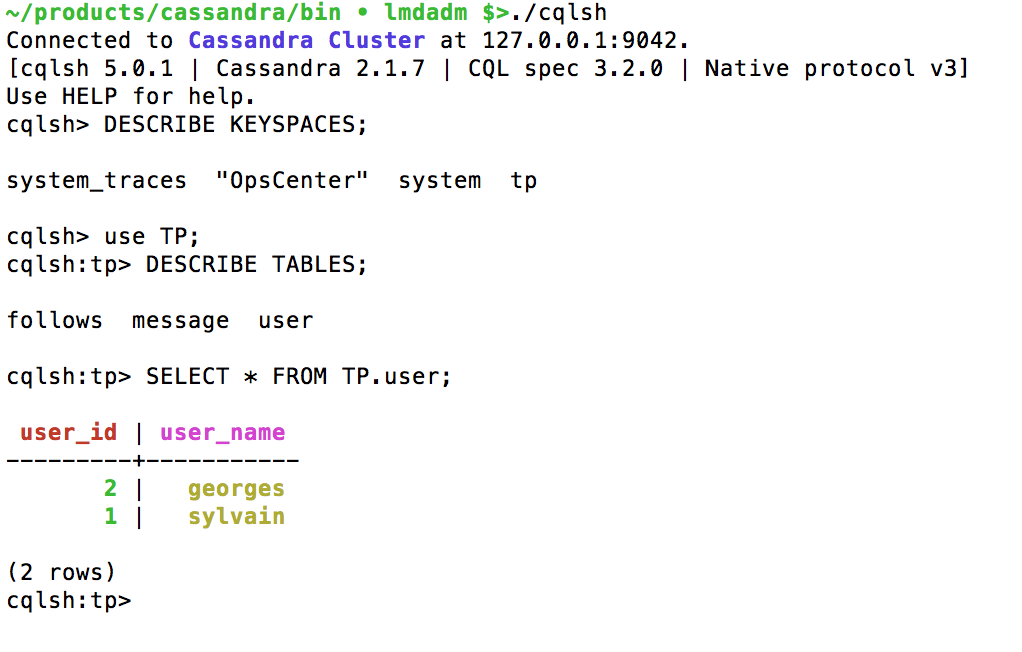
\includegraphics[scale=0.5]{img/cqlsh.png}
\caption{Quelques commandes cql.}
\end{figure}

\subsection{le CQL, langage de requête Cassandra}


\par 
\begin{block}{remarque}
On note que l\rq utilisation de double quotes (") dans la ligne de commande provoque l'erreur: \newline
\begin{tt}
\textcolor{red}{
SyntaxException: <ErrorMessage code=2000 [Syntax error in CQL query]
message="line 1:58 extraneous input hello world expecting ) (...) values (1,1 hello world[)]...)>
}
\end{tt}
\end{block}

\subsection{Clefs composites}
Via Devcenter on insert les lignes demandées comme sur les figures suivantes. \newline
\begin{figure}[h!]
\centering
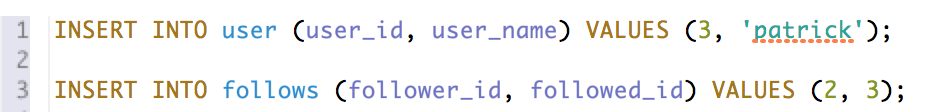
\includegraphics[scale=0.7]{img/add_patrick.png}
\caption{Ajout de l'utilisateur patrick suivit par georges.}
\end{figure}

Puis on vérifie la table des relations d'abonnement \lq follows\rq.
La premier relation d'abonnement (georges suit sylvain) à été supprimée.
En effet, lors de la définition de la famille de clef follows, la colonne
follower\_id est déclarée comme une clef primaire, elle est donc unique. Autrement dit
On ne peut suivre qu'une seule personne à la fois.
\begin{figure}[h!]
\centering
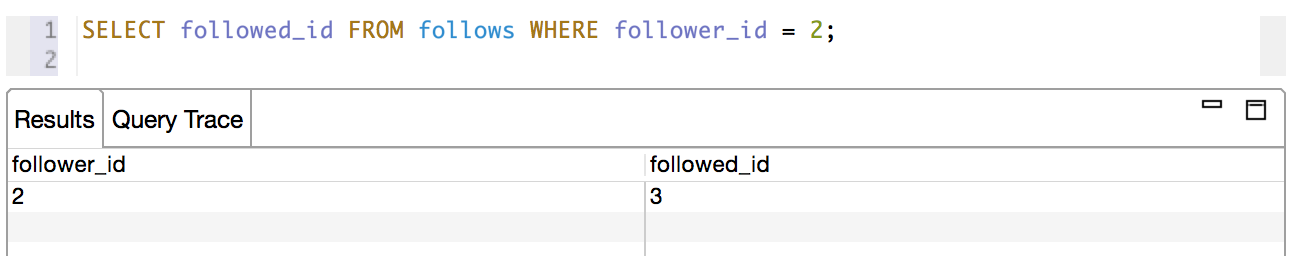
\includegraphics[scale=0.6]{img/solo_key.png}
\caption{Unique relation de la table follows après l'ajout de patrick.}
\end{figure}


